%!TEX root = ../master.tex
\section{Burglar}
This section provides an analysis of an attack in which a burglar wants to break in to the house of the consumer and steal his valuables.
Several options to achieve this goal are explored.
These are listed below:
\begin{itemize}
  \item \Cref{attacktree:burglar:sm}: Compromising the security on the smart meter.
  \item \Cref{attacktree:burglar:client}: Compromising the device (the client) the consumer is using to communicate with the smart meter.
  \item \Cref{attacktree:burglar:ecm}: Installing an ECM (see \cref{ecm}) and monitoring the consumer.
  \item \Cref{attacktree:burglar:physical}: Performing a \emph{``physical''} attack, involving no technology.
\end{itemize}

Representing the attacks as four separate attacks might be somewhat misleading.
For instance the burglar might choose a physical means of determining if the consumer is at home even though he initially compromised the smart meter.
Thus the four attack trees might be combined to properly describe the full spectrum of the burglars attack strategies.

The trees are represented as four trees here to show the correlation between how the burglar gains access to the system and the possible attacks this makes available.
The separated trees provide a clear visualization of this relation.

This representation is to used to build a model of the possible threat to the consumer.
As this representation fails to fully represent attacks that employ multiple strategies, special care should be taken when modeling the trees.
Using a model that joins the four trees will allow for a comparison of the validity of the each device as an entry point for an attack.

\begin{figure}
\center
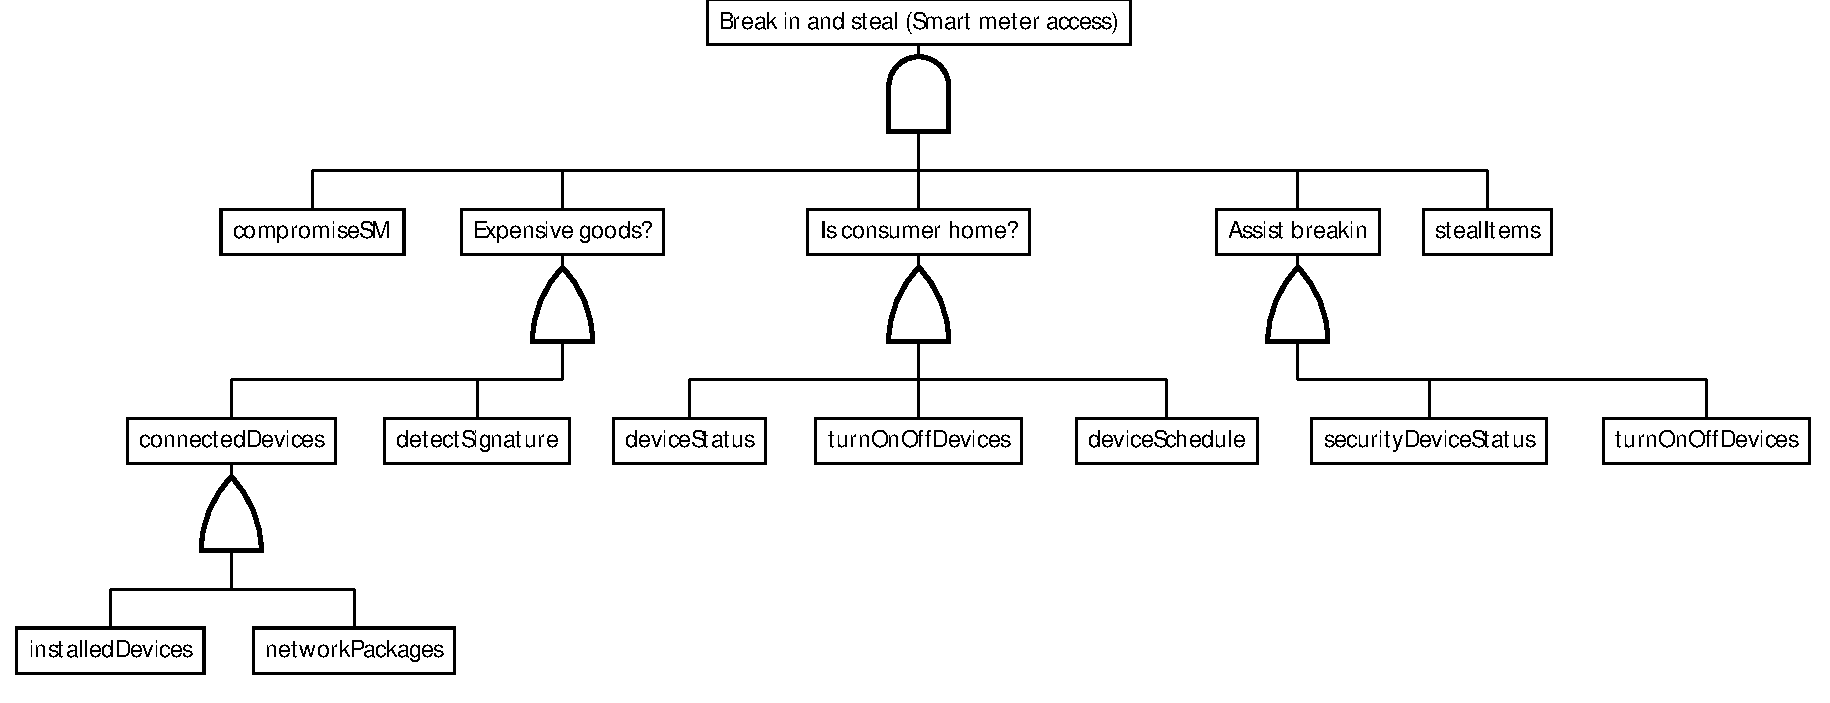
\includegraphics[width=\textheight, angle=90]{graphviz/burglarSM.pdf}
\caption{Attack-tree of a burglar attacking the consumer using the smart meter.}
\label{attacktree:burglar:sm}
\end{figure}

\begin{figure}
\center
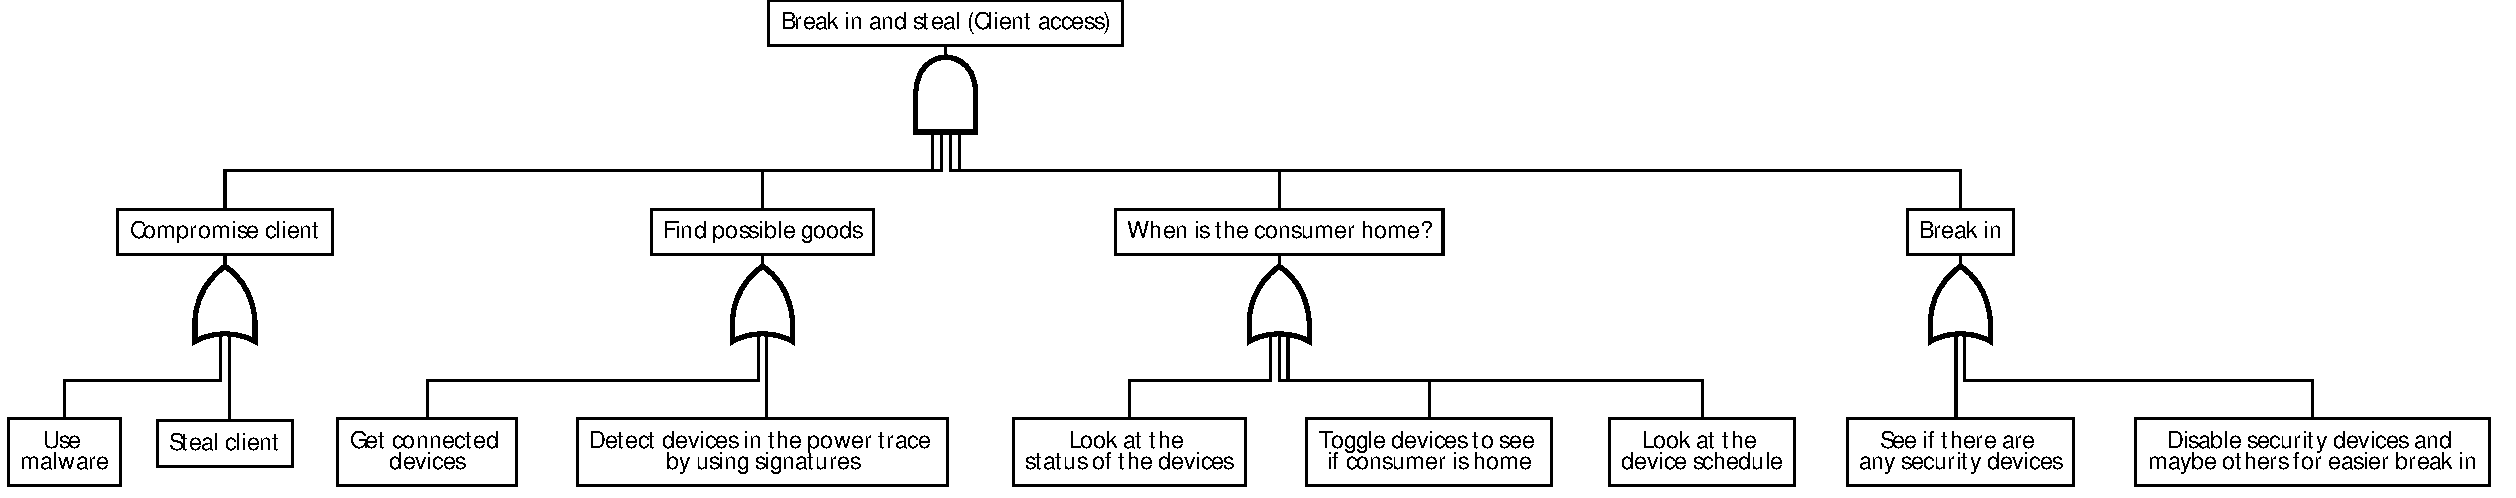
\includegraphics[width=\textheight, angle=90]{graphviz/burglarClient.pdf}
\caption{Attack-tree of a burglar attacking the consumer using the consumers client.}
\label{attacktree:burglar:client}
\end{figure}

\begin{figure}
\center
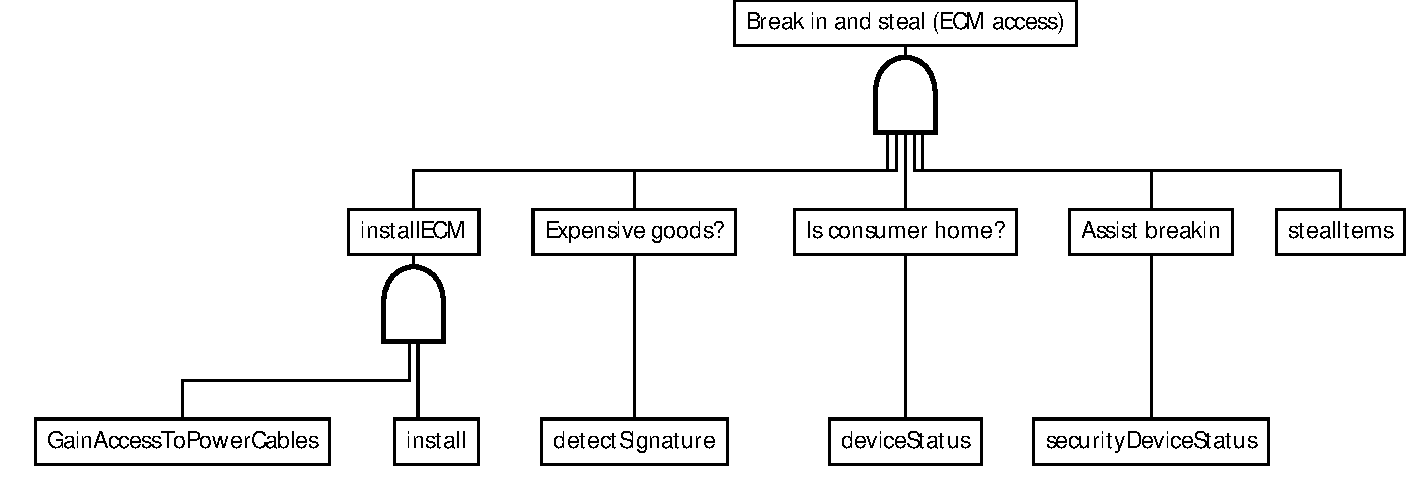
\includegraphics[width=\textheight, angle=90]{graphviz/burglarECM.pdf}
\caption{Attack-tree of a burglar attacking the consumer using an ECM.}
\label{attacktree:burglar:ecm}
\end{figure}

\begin{figure}
\center
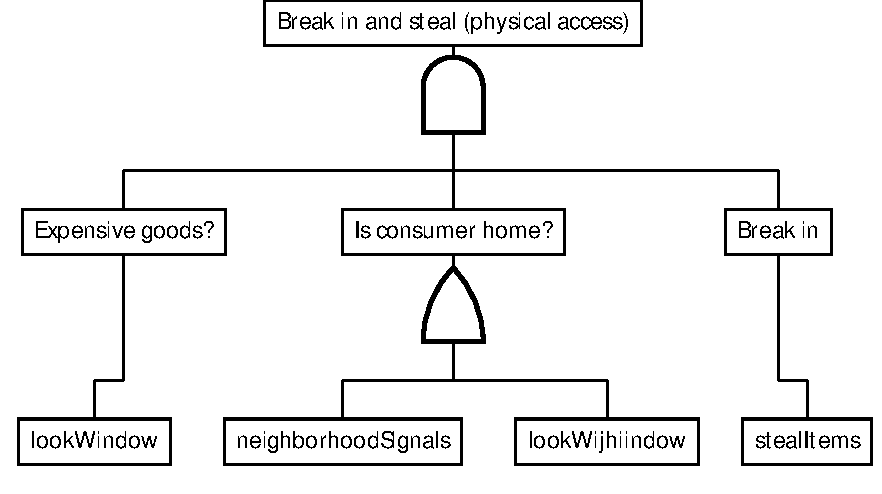
\includegraphics[width=\textheight, angle=90]{graphviz/burglarPhysical.pdf}
\caption{Attack-tree of a burglar attacking the consumer through physical means.}
\label{attacktree:burglar:physical}
\end{figure}

\subsection{Gaining access}
In order to access information about the power consumption of the consumer, the burglar needs to gain access to either the smart meter, a consumer device that controls the smart meter or install an ECM unit (see \cref{ecm}).

\subsection{Expensive goods}
The first step for the burglar is to determine if anything is of value in the house. 
The burglar can choose any house he wants, so he will probably access the house which will yield the highest total worth for the least effort.

The physical method is simply to look in through windows of the house and consider what can be seen. 
This method has some obvious shortcomings.
Not everything can be seen from the outside, and in multiple story houses several stories may be impossible to evaluate.
Is is also rather inaccurate -- it may be possible to see a TV, but is it the newest product from this year, or is it an older model that is virtually impossible to sell?

If the burglar has compromised either the smart meter, or the internet router of the consumer, he will be able to find out what products are in the home. 
This is possible either through some smart meter database that shows what can be controlled, or through network traffic which can indicate what products are being communicated with.

If the burglar has access to the power consumption (either smart meter or the ECM), it will be possible to detect product signatures in this data, see \cref{smart_meter_privacy}.
This is difficult and possibly ambiguous, but it may provide pointers on what he can expect to find.

\subsection{Is the consumer at home?}
When the burglar decides on a home to be his target he needs to plan when to break in.
Before doing that he needs information about when the consumer is home.

Again, he can use some physical methods to determine this.
He can look through the windows to check for activity in the house.
This technique is not guaranteed to show that he is not a home, but if there is activity the burglar can be sure that he is at home.
Over a longer period of time this technique can provide information about the habits and work hours of the consumer, making it easier to plan when to break in and when to be out again.

Another technique is to put indicators in the neighbourhood.
This could be small signs on the mailbox, a can behind the tire of a car, or a knocked over bike.
The purpose of these subtle indicators is to find out if someone is not home for a longer period of time.
If the consumer is home he will with great probability set up the bike or remove the mark from the mailbox.
But if he is not at home the burglar will be able to see this from the indicator.
This technique works particularly well if the burglar has several targets in the neighbourhood, because he can just choose the house that has no activity.

If the burglar has access to the smart meter or an ECM (External Consumption Meter) he has some options that can help him determine if the consumer is at home.

From the power consumption it would be possible to determine what devices are currently on. 
If the TV is turned on and off in irregular intervals (timers exist that can turn devices on and off at predetermined intervals), it is an indicator that he is home.

Also, schedule information can be an indicator if he is at home.
If the consumer schedules laundering during the night it must indicate that he plans to be home some time after the ended laundering.
The schedule may also provide information about work hours of the consumer, making it possible for the burglar to plan the break in.

Having control over the smart meter also provides the power to turn devices on or off.
The burglar can use this to reinforce any suspicion he has that the consumer is, or is not, home.
If he thinks that the TV is turned on by some timer mechanism he can force it to turn off.
If the consumer is really at home he will probably turn it on again.
Provided that this action must be done manually, this is a sure-fire proof that he is at home.
Another test could be to turn the stereo on and put the volume to an abnormally high level.
If the consumer does not react to this, he is either sleeping very tight or not at home.

\subsection{Break in}
When the burglar feels confident that he wants to break into the house he can use the smart meter for some additional help.
The smart meter can provide information about the security status of the house.
If there is a security-alarm or -camera, this will be visible on the smart meter by the same techniques mentioned in the ``Expensive goods'' sub-tree -- either in the consumption data, network data, or smart meter database.
If the consumer has some security devices installed he can turn them off entirely and make the break in easier without even entering the property.

The last step is to steal all the expensive goods in the house of the consumer.
The smart meter (as well as surveillance) can have provided information that can tell the burglar when the consumer is usually home, and he therefore know when to be out in order to not get caught.
